%% this formatting courtesy of https://github.com/jgabry/qmss_paper/blob/master/thesis.tex

\documentclass[oneside,12pt] {book}

% MARGINS: one inch
\usepackage[margin=1in]{geometry}

% DOUBLE SPACING
\renewcommand{\baselinestretch}{2}
\usepackage{setspace}
\usepackage{etoolbox}
\usepackage{setspace}
\usepackage{todonotes}
\usepackage{fullpage}
\usepackage{graphicx}
\usepackage{amsfonts}

\usepackage[]{hyperref}
\hypersetup{
    pdftitle={Some Bullshit},    % title
    pdfauthor={Simon Rimmele},     % author
    colorlinks=true,       % false: boxed links; true: colored links
    linkcolor=black,          % color of internal links (change box color with linkbordercolor)
    citecolor=black,        % color of links to bibliography
    filecolor=black,      % color of file links
    urlcolor=black           % color of external links
}



\graphicspath{{assets/}}


% APA CITATIONS
\usepackage[bibnewpage, nosectionbib]{apacite} %apa citation style
\bibliographystyle{apacite}

% FONTS
\usepackage[]{mathptmx}
\usepackage{amsmath,amsfonts,amssymb}
\usepackage{bm} % Bold-italic math font

% ALIGNMENT & INDENTATION
\usepackage[document]{ragged2e} % left alignment (ragged right) instead of justified
\setlength{\RaggedRightParindent}{.5in} % 1/2 inch paragraph indentation
\usepackage{indentfirst} % indent first paragraphs after \section{} and friends

% APPENDICES
\usepackage[toc,title,page]{appendix}

% FOR FIGURES
\usepackage{graphicx}
% FOR LISTS
\usepackage{enumerate}

% FOR NICER TABLES
\usepackage{booktabs}

% FIGURE CAPTIONS
\usepackage[font={small, it},format=hang,justification=justified,labelsep=space,labelfont={small,bf,up}]{caption}

% SIDE-BY-SIDE FIGURES
\usepackage{subcaption}

% CHAPTER TITLE STYLES
\usepackage{titlesec}
\definecolor{gray75}{gray}{0.75}
\newcommand{\hsp}{\hspace{20pt}}

% % PRETTY FORMATTING OF SOURCE CODE
% \usepackage{styles/lstBUGS} % for pretty source code (https://github.com/jrnold/lstBUGS)
% \lstset{
% basicstyle=\scriptsize\singlespacing,
% keywordstyle=\color{DarkSlateGray}\bfseries,
% keywordstyle=[2]{\color{Black!80}},
% commentstyle=\color{DimGrey},
% frameround=fttt,
% backgroundcolor=\color{AliceBlue!80},
% xleftmargin=2em,
% xrightmargin=2em
% }

% HEADER, FOOTER, PAGE NUMBERS
\usepackage{fancyhdr} %header
\pagestyle{fancy}
\fancyhf{}
\renewcommand{\headrulewidth}{0pt} % remove line at top of each page
\fancyfoot[R]{\thepage} % Set the right side of the footer to be the page number

\fancypagestyle{plain}{% Redefine plain style, which is used for titlepage and chapter beginnings
    \renewcommand{\headrulewidth}{0pt}% From http://tex.stackexchange.com/a/30230/828
    \fancyhf{}%
    \fancyfoot[R]{\thepage}%
}

% FIGURE CAPTIONS
\usepackage[font={small, it},format=hang,justification=justified,labelsep=space,labelfont={small,bf,up}]{caption}

%CHAPTER TITLE STYLES
\usepackage{titlesec}
\definecolor{gray75}{gray}{0.75}
\newcommand{\hsp}{\hspace{20pt}}



% TITLE PAGE
\newcommand*{\titleGM}{\begingroup % Create the command for including the title page in the document
\hbox{ % Horizontal box
\hspace*{0.2\textwidth} % Whitespace to the left of the title page
\rule{1pt}{\textheight} % Vertical line
\hspace*{0.05\textwidth} % Whitespace between the vertical line and title page text
\parbox[b]{0.75\textwidth}{ % Paragraph box which restricts text to less than the width of the page

\singlespacing
{\noindent\Huge\bfseries A Good Title}\\[2\baselineskip] % Title
{\large \textit{blah blajh blah }}\\[4\baselineskip] % Tagline or further description

\vspace{2cm}

{\LARGE \textsc{Simon Rimmele}} % Author name

\vspace{.5cm}

{\large \textsc{Advisor: Benjamin Goodrich}}

\vspace{.5cm}
\textsc{May, 2018}

\vspace{0.3\textheight} % Whitespace between the title block and the publisher
\begin{center}
%{\noindent \bf }\\[\baselineskip]
{\noindent Columbia University $\vert$ New York}
\end{center}
}}
\endgroup}
% end TITLE PAGE



\begin{document}

\titleGM % This command includes the title page


\begingroup
\mainmatter

\chapter{Introduction}
\label{introduction}

Urban areas produce vast amounts of data each day, much of it bound to specific location and time. Every bus signaling its location to an app, every complaint made about noisy neighbors, every police report about a traffic collision is a measurement. While it is easier than ever to put data on a map, making sense of it as an administrative or policy professional can be an exercise in frustration. Answers to simple questions about why things are happening and where they may happen next typically require statistical knowledge and access to even more explanatory data. \par

There is potential for explanatory or predictive modelling using solid statistical foundations and only the data at hand. Some progress in this direction has been made when considering timeseries; Facebook's Prophet is a successful forecasting tool with a Bayesian underpinning that nevertheless is accessible to analysts and researchers who bring their own skillset and expert knowledge \cite{prophet}. To use Prophet all one has to do is bring a timeseries and potentially some prior guesses about trends or important events. The additive model underpinning Prophet is capable of neatly decomposing the timeseries into multiple interpretable trends and also offers forecasting under uncertainty. \par

Using space as a predictive dimension in the same way Prophet uses time has the potential to be immensely helpful for urban research and administration. There is obvious theoretical and practical appeal to using spatiotemporal methods in the context of the 'Smart City', whose premise is found in rethinking urban areas as an intricate system monitored and managed at a previously impossible level of detail through the use of data \cite{kitchin_2014}. While Smart City proponents have pointed to the potential of technological data generating mechanisms such as sensor networks, there is already a vast amount of generated data available through administrative channels such as 311, public safety reporting, or existing networked sensor systems like traffic monitoring. While there have been limited surveys into the use of spatiotemporal models for urban applications, even these were restricted to forecasting at a low level of spatial granularity such as load demand for energy grids \cite{tascikaraoglu_2017}. Little work has been done to assess the viability of making use of hyperlocal data for forecasting outcomes in an urban environment, much less productionizing a model to better deliver social services exactly where they are needed and at the right time.


\chapter{Literature \& Model Review}
\label{literature_review}

\section{Spatiotemporal Modelling}

Count-based spatial and spatiotemporal models are widely used in ecological fields e.g., for wildlife population and habitat studies \cite{cobi_2008}, as well as in the public health field for disease mapping \cite{schrodle_2011}. Intrinsic  Conditional AutoRegressive models (ICAR) are a spatial-only model with widespread application in public health context and produce a measure of relative risk similar to the one used for this project \cite{wakefield2006disease}.   Spatial and spatiotemporal models used in these fields are typically at a low to medium level of spatial granularity, such as the regional model of the northwestern United States used in \cite{cobi_2008}. For studies set in urban areas some research has been done at the level of census tracts in an individual county, like Chun et., al's study on disparities in environmental hazards in Maricopa County \cite{chun_2012}. \par

Outside of the natural and environmental sciences, some forms of spatial and spatiotemporal modelling have found use in predictive policing research and industry use, given that "space–time interactions are deeply embedded both empirically and theoretically into many areas of criminology" \cite{li_2014}. The scope of police work also dictates most or all predictive modelling is done in urban areas and at a much finer scale of spatial granularity. Recently developed likelihood-based estimators for spatiotemporal counts have been fit on crime data from 138 census tracts in Pittsburgh, Pennyslyvania \cite{liesenfeld_2017}; Flaxman et. al., developed a forecasting algorithm for crime in Portland, Oregon at the granularity of 66,000 cells measuring a quarter of a square mile each \cite{flaxman_2018}.
 \par

Other than in law enforcement, spatiotemporal models have also found some applications in urban social science through traffic modelling. Cheng et. al., used a non-Bayesian approach to model and forecast traffic dynamics in London \cite{cheng_2012}. In this study, the authors pose and attempt to grapple with one of the fundamental and ongoing challenges of using data in the context of a Smart City; the volumes of data available are often so massive thay they either overwhelm existing modelling methods and/or offer an almost endless number of ways to further segment and structure the data for use. Cheng et. al, use a variety of non-Bayesian methods including likelihood-based statistical models and gradient-based neural networks, but find these methods incapable of capturing the full autocorrelation structure of traffic networks. The tradeoff between the spatiotemporal complexity of a model and the computational feasibility of fitting the model in medium to large datasets is evident here. \par



\section{Gaussian Processes}

This project will assess the viability of using Gaussian Process models for spatiotemporal predictions in urban settings. Gaussian Processes have attractive properties for sparse data because a model can be interpreted as interpolating an unobserved point between known distributions. As mentioned in the literature review, spatiotemporal models have historically suffered from computational infeasibility when the amount of data as well as spatial and temporal dimensionality grows. Recent advances in Bayesian probablistic programming and implementations of Gaussian Processes that take advantage of the relative sparsity of data across spatial dimensions has reduced the computational burden of fitting these models. \par

A Gaussian Process (GP) is a generalization of a Gaussian - also known as the Normal - distribution. A Normal distribution is defined by a scalar mean $\mu$ and variance $\sigma$ in the univariate case, and a n-length vector $\mathbf{\mu}$ with a n-by-n dimensional covariance matrix $\Sigma$ in the multivariate case. A Gaussian Process ''can be viewed as a potentially infinite-dimensional generalization of [the] Gaussian distribution'' \cite{gelman2013bayesian} , p. 501. However any finite-dimensional marginal distribution from a Gaussian Process is also Gaussian, which makes a GP suited as a prior distribution for some unknown regression function $\mathbf{\mu}(x)$ - where $x$ is a vector with arbitary but finite dimensions. A generic Gaussian Process $\mu \sim GP(m,k)$ is a series of random functions drawn from an n-dimensional normal distribution \cite{gelman2013bayesian}: \par

$$ \mu(x_1),...,\mu(x_n)) \sim N((m(x_1),...,m(x_n)),K(x_1,...,x_n)) $$

Thus a Gaussian Process is defined entirely by a mean function $m$ and covariance function/s $K$. Sums and products of GPs are also GPs, which makes it simple to combine different variations of covariance functions.

\subsection{Estimating Gaussian Processes}

While it is not necessary to go into extensive detail about the theory of Gaussian Processes for this application, it is relevant to briefly describe what part of the estimation poses a challenge for high-dimensional datasets like those found in spatiotemporal forecasting. To generate samples from a finite-dimensional realization of a GP $\mathbf{\mu} \sim N(\mathbf{m},K)$, it is necessary to calculate the Cholesky decomposition of the covariance matrix: $K=LL^\intercal$. Then it easy to generate standard Normal draws $\mathbf{u} \sim N(\mathbf(0),I)$, and shift them using $\mathbf{\mu}=\mathbf{m}+L\mathbf{u}$ \cite{rasmussen_2005}. Calculating $L$ is quite computationally demanding as $n$ rises. In practice the eigenvalues of $K$ can also decay, causing the decomposition to fail. This is solved in practice by adding a small 'jitter' term to the diagonal of $K$. Ideally the jitter term is small enough to not influence the estimates, but this has to be assessed through trial and error. \par


\section{The Log-Gaussian Cox Process}

Log-Gaussian Cox Process (LGCP) models are a further extension of a Gaussian Process with particular applicability to prediction of count data. A LGCP is hierarchical in that the data are assumed to be drawn from a Poisson likelihood with intensity parameter $\lambda$. The Poisson likelihood function has theoretical properties suitable for relatively sparse count (integer) data which makes it appealing for use in modelling frequent events that are nevertheless sparse when segmented over space and time dimensions. In turn the log of $\lambda$  is generated by a Gaussian process\cite{teng_2017}. This makes the LGCP quite flexible in inputs and dimensionality while also making model fitting generally computationally burdensome. \par

An alternative specification uses a Gaussian likelihood, which has the added appeal of making the likelihood and prior conjugate to each other and solvable in closed form. As the $\lambda$ parameter of a Poisson distribution increases the distribution converges to a Normal distribution anyway, so this model may be more applicable to situations when counts are not sparse e.g., at lower granularities of space and/or time, which was not considered in detail here.

A zero-inflated Binomial (ZIB) likelihood would be another alternative to consider for this type of modelling. As the name implies, a ZIB distribution has a higher probability density around zero and may be better suited for extremely sparse data like gridded observations with very small grid dimensions.

 The general model follows the specification and notation used by "A General Approach to Prediction and Forecasting Crime Rates with Gaussian Processes" \cite{flaxman_2014}: \par


$$\lambda(s,t) = exp((s,t))$$

$$ y_{s,t} | \lambda(s,t) \sim Poisson(exp(f(s,t))e_s) $$

The outcome count $y_{s,t}$ at location $s$ and time $t$ is generated from a Poisson distribution whose scale parameter is a the function $f(s,t)e_t$. $f(s,t)$ is a function with a Gaussian process prior, while $e_s$ is a fixed spatial expectation term $\mathbb{E}[y_s]$. The spatial expectation is a convenient way to incorporate prior information about the variable of interest. Again following Flaxman 2014, using an exponential link function gives a practical interpretation of $exp(f(s,t))$ as the relative risk function while $f(s,t)$ itself is the log-relative risk. When the log-relative risk is 0, the relative risk is 1 and the expected value of of the outcome $y(s,t)$ is just the prior spatial expectation $e_s$. Finally, every count outcome $y_{s,t}$ is assumed independent conditional on $f$, so the joint conditional likelihood of all $y$ factors as a product.

$$p(y|f) = \prod_{s,t}{ Poisson( y_{s,t}| exp(f(s,t))e_s)}$$

\subsection{f(s,t)}

$f$ is modeled as following a generic Gaussian process with a mean of zero and a covariance matrix $K$:

$$ f \sim GP(0,K) $$

Spatiotemporal elements enter the Gaussian process model through $K$, which is used to capture the relationships of interest and entirely determines the model. Since variance/covariance is additive, any variance term can be decomposed at least theoretically into arbitrarily many additive components. Purely spatial and temporal elements as well as interactions can be incorporated using different kernel functions, and different combinations of kernels may produce more accurate results. Cross-validating models with different types and combinations of kernel functions will help identify the specification with the best predictive properties. Since the cross-validation data are correlated in this model the cross-validation set will have to be drawn from spatially contigous representative subsets of the data.

\subsection{Kernels}

There are a wide variety of existing kernel functions documented for use in Gaussian process models \cite{rasmussen_2005} and it is also possible to define custom functions as long as they follow certain properties. The entirety of a GP is determined by its kernel/s, which makes them versatile and open to many different specifications. \par

An important consideration is whether the model is considered to be stationary. In spatiotemporal models the case for assuming stationarity weakens as the time-period being considered lengthens, and this should in turn affect the kernel choice. The long term model considered includes a non-stationary linear kernel component intended to capture any long-term trends:    \par

\begin{itemize}
  \item $k_t(t)$ : a temporal kernel
  \item $k_p(t)$ : a periodic kernel
  \item $k_l$: a linear kernel
\end{itemize}

The short-term models considered for this project are all stationary and loosely follow Flaxman 2014 by consisting of up to four individual kernels $k$ , where $K=\sum_{i}k_i$. The four basic kernel types were:

\begin{itemize}
  \item $k_s(s)$ : a spatial kernel
  \item $k_t(t)$ : a temporal kernel
  \item $k_p(t)$ : a periodic kernel
  \item $k_{st}(s,t)$ : a space-time interaction kernel
\end{itemize}

Radial Basis Function (RBF) and Matern family kernels are both candidates for spatial and temporal modelling. Their point of differntiaion lies in the extent to which they 'smooth' the input. The most appropriate kernel will vary based on the characteristics of the observations being modeled.

The RBF kernel - also called the squared exponential - is widely used as a default stationary kernel:

$$ k_t(t) = exp\big(- \frac{(|t-t'|)^2}{2\ell^2}\big) $$

The L1 norm $|t-t'|$ of the input determines the kernel, along with $\ell$,  a lengthscale parameter that is common to kernel functions.

The Matern family kernels are defined:

$$ k_t(t) = \frac{1}{2^{\nu - 1}\Gamma(\nu)}\big(\frac{\sqrt{2\nu}}{\ell}(|t-t'|)\big)^\nu K_{\nu}\big(\frac{\sqrt{2\nu}}{\ell}(|t-t'|)\big)$$

The parameter $\nu$ determines the degree of smoothness and the kernel converges to a Gaussian kernel as $\nu$ goes to $\inf$. Typical values of $\nu$ are fractions,with $\nu=\frac{1}{2}$ or $\frac{3}{2}$ being quite common. The name of a specific kernel is often expressed by referencing the parameter value, so in this paper a 'Matern32'  refers to a Matern kernel with $\nu=\frac{3}{2}$. Figure \ref{kernel_examples} shows a comparison of the degree of smoothing a RBF,Matern12, and Matern32 kernel have on the same multivariate random input:

\begin{figure}[h!]
  \centering
  \caption{A comparison of RBF with Matern family kernels.}
  \label{kernel_examples}
  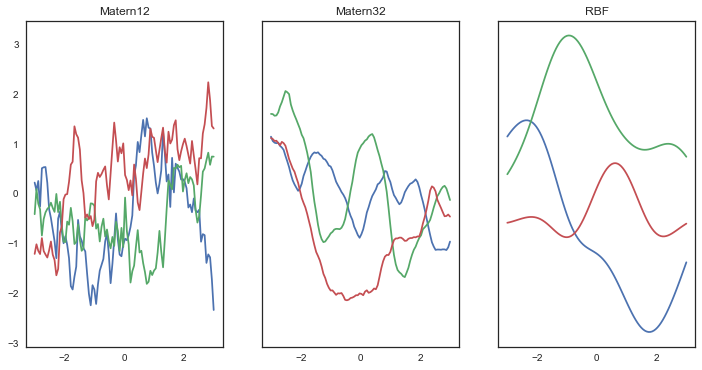
\includegraphics[width = 0.8\textwidth]{kernel_examples}
\end{figure}


The periodic is another class of stationary kernel. The variant used in this project follows MacKay 1998  \cite{mackay1998introduction}:

$$ k_p(t) = exp \bigg[ - \frac{1}{2}\sigma_i \big(\frac{sin(\frac{\pi}{\Delta}(t_i - t_i'))}{\ell} \big)^2 \bigg] $$

$\Delta$ is a periodicity paramter that can either be fit or set to a fixed anticipated value such as 52 for annual weekly data. $\ell$ is again the lengthscale parameter.\par


\subsection{Priors}

Gelman 2006 suggests using a student-t prior distribution restricted to be positive (a 'half-t') as a prior for variance parameters in hierarchical models \cite{gelman_2006}. Since variance is always positive it is acceptable and desirable to restrict the prior distribution to be non-negative as well. Flaxman 2014 used a standard student-t prior with 4 degrees of freedom on all parameters (not just variance). Both standard Normal $N \sim (0,1)$ and Student-T priors were considered here. The normal prior has less probability mass in its tails than the Student-t but is otherwise a close substitute. The Normal prior did sometimes lead to the optimization algorithm failing to find a credible set of parameter estimates, while the Student-T with degrees of freedom between 2 and 10 performed better. Increasing the variance on the prior distributions was another way to lower the probability of the optimizer failing, but it also led to dramatically increased runtimes in some cases.

\section{Methods for fitting LGCPs}

Solutions to the computational challenges in fitting LGCPs have advanced rapidly over the past five years. As mentioned earlier, the computational bottleneck for Gaussian Process models is the the n-by-n covariance matrix, which requires an $O(n^3)$ computation. Fitting a GP model as $n$ grows beyond a few thousand points is quite challenging \cite{gelman2013bayesian}. \par

 As recently as 2012 the best methods for fitting LGCP models involved variations of the Metropolis-Hastings sampling algorithm which were considered to be slow and highly inefficient in generating acceptable draws from the posterior distribution of the model \cite{murray_2012}. Advances in statistical computing have opened the door for several new model fitting methods, each with their own advantages and drawbacks.

\subsection{Variational Inference}

Variational Inference (VI) methods attempt to recover parameter estimates for a posterior distribution of interest by specifying a more tractable family of distributions and optimizing the resulting approximation using closed-form or computational methods. Usually the family of approximating distributions is denoted $Q$, and the optimization seeks to minimize the Kullback-Leiber divergence $KL[(\theta), p(\theta|y)]$ between $q(\theta)$ and the true posterior $p(\theta|y)$. \par

In the case of the LGCP with Poisson likelihood there is no direct closed-form solution because an intractable integral is involved. VI methods have in the past been limited by needing to make simplifying assumptions about the approximating distributions. Usually VI makes the 'mean-field' assumption (borrowed from physics), that the posterior can be approximated by the product of some number of existing distributions: $q(\theta_1,...,\theta_n)= \prod_j{q_j(\theta_j)}$. The mean-field assumption is especially unsuited for high-dimensional models like a Gaussian Process, but Tran and Blei characterize a Variational Gaussian Process method that avoids the assumption \cite{tran_2015}. GPflow - the package used for this project - uses the Variational Gaussian  for fitting \cite{GPflow2017}.\par

The major drawback of variational methods is there are no theoretical justifications for the accuracy of estimates produced because it is unclear and often unknowable how close the optimized approximation is to the true posterior distribution, where the $KL$ divergence term is a unitless and uninterpretable difference between the two that cannot be compared across models. Yao et., al. recently proposed Pareto-Improved-Importance-Sampling (PSIS) and Variational-Simulation-Based-Calibration (VSBC) methods for assessing whether a VI approximation ''worked'' \cite{yao_2018}.

\subsection{MCMC}

Markov Chain Monte Carlo (MCMC) sampling methods by contrast do have theoretical properties that ensure consistent estimation of the posterior distribution - at least  as the numbers of samples increases asympotically \cite{teng_2017}. MCMC methods are not a new development in themselves, but there have been breakthroughs both in MCMC algorithm design and computing power required to fit more complex models. The probablistic programming language Stan has been used for spatiotemporal modelling of causes of mortality using Gaussian Markov Random Field models, another potential alternative to LGCPs that may be appropriate for urban forecasting but are not considered here \cite{stan} \cite{foreman_2017}. In contrast to VI, MCMC also is capable of producing estimates for full posterior distributions for parameters of interest, rather than point estimate approximations. In the case of urban prediction and forecasting, access to full posterior estimates would offer much more probalistic information from which to draw uncertainty-based conclusions in a policy or administrative context.

\subsection{LaPlace Approximation}

Integrated Nested LaPlace Approximation (INLA) is an alternative to MCMC capable of fitting a LGCP \cite{illian_toolbox}. INLA works by approximating the distribution of each parameter around the mode of its posterior \cite{lindgren2015bayesian}. The marginal posteriors are calculated by numerically integrating over the parameters, followed by another approximation of the marginal posterior (hence the 'Nested' component of INLA). When the number of hyperparameters is relatively small, INLA is capable of quickly fitting a latent Gaussian field model - of which the LGCP is a special case \cite{rue2009approximate}. LGCP models usually assume a square grid structure for the spatial component in order to fit the model, but Simpson 2016 also fits LGCPs without relying on explicit grid structure \cite{simpson2016going}.


\section{Method Choice}

MCMC methods clearly offer desirable properties superior to VI methods, and full MCMC models similar to the ones considered here have been explored \cite{Flaxman2015FastHG}. However, their practical limitations made them somewhat burdensome to consider for this project. The most unfortunate drawbacks were that MCMC is very slow to fit in comparison with VI. In an attempt to draw a compromise between ease of experimentation and model reliability this project used VI methods under the knowledge that they may not produce the best results for practical use. Simple posterior checks were done to assess the results.


\chapter{Research Design}
\label{design}


This project will assess the viability of using Gaussian Process models for spatiotemporal predictions in urban settings. Gaussian Processes have attractive properties for sparse data because a model can be interpreted as interpolating an unobserved point between known distributions. As mentioned in the literature review, spatiotemporal models have historically suffered from computational infeasibility when the amount of data as well as spatial and temporal dimensionality grows. Recent advances in Bayesian probablistic programming and implementations of Gaussian Processes that take advantage of the relative sparsity of data across spatial dimensions has reduced the computational burden of fitting these models. \par


\section{Gaussian Processes}

A Gaussian Process (GP) is a generalization of a Gaussian - also known as the Normal - distribution. A Normal distribution is defined by a scalar mean $\mu$ and variance $\sigma$ in the univariate case, and a n-length vector $\mathbf{\mu}$ with a n-by-n dimensional covariance matrix $\Sigma$ in the multivariate case. A Gaussian Process ''can be viewed as a potentially infinite-dimensional generalization of [the] Gaussian distribution'' \cite{gelman2013bayesian} , p. 501. However any finite-dimensional marginal distribution from a Gaussian Process is also Gaussian, which makes a GP suited as a prior distribution for some unknown regression function $\mathbf{\mu}(x)$ - where $x$ is a vector with arbitary but finite dimensions. A generic Gaussian Process $\mu \sim GP(m,k)$ is a series of random functions drawn from an n-dimensional normal distribution \cite{gelman2013bayesian}: \par

$$ \mu(x_1),...,\mu(x_n)) \sim N((m(x_1),...,m(x_n)),K(x_1,...,x_n)) $$

Thus a Gaussian Process is defined entirely by a mean function $m$ and covariance function/s $K$. Sums and products of GPs are also GPs, which makes it simple to combine different variations of covariance functions.

\subsection{Estimating Gaussian Processes}

While it is not necessary to go into extensive detail about the theory of Gaussian Processes for this application, it is relevant to briefly describe what part of the estimation poses a challenge for high-dimensional datasets like those found in spatiotemporal forecasting. To generate samples from a finite-dimensional realization of a GP $\mathbf{\mu} \sim N(\mathbf{m},K)$, it is necessary to calculate the Cholesky decomposition of the covariance matrix: $K=LL^\intercal$. Then it easy to generate standard Normal draws $\mathbf{u} \sim N(\mathbf(0),I)$, and shift them using $\mathbf{\mu}=\mathbf{m}+L\mathbf{u}$ \cite{rasmussen_2005}. Calculating $L$ is quite computationally demanding as $n$ rises. In practice the eigenvalues of $K$ can also decay, causing the decomposition to fail. This is solved in practice by adding a small 'jitter' term to the diagonal of $K$. Ideally the jitter term is small enough to not influence the estimates, but this has to be assessed through trial and error. \par


\section{The Log-Gaussian Cox Process}

Log-Gaussian Cox Process (LGCP) models are a further extension of a Gaussian Process with particular applicability to prediction of count data. A LGCP is hierarchical in that the data are assumed to be drawn from a Poisson likelihood with intensity parameter $\lambda$. The Poisson likelihood function has theoretical properties suitable for relatively sparse count (integer) data which makes it appealing for use in modelling frequent events that are nevertheless sparse when segmented over space and time dimensions. In turn the log of $\lambda$  is generated by a Gaussian process\cite{teng_2017}. This makes the LGCP quite flexible in inputs and dimensionality while also making model fitting generally computationally burdensome. \par

An alternative specification uses a Gaussian likelihood, which has the added appeal of making the likelihood and prior conjugate to each other and solvable in closed form. As the $\lambda$ parameter of a Poisson distribution increases the distribution converges to a Normal distribution anyway, so this model may be more applicable to situations when counts are not sparse e.g., at lower granularities of space and/or time, which was not considered in detail here.

A zero-inflated Binomial (ZIB) likelihood would be another alternative to consider for this type of modelling. As the name implies, a ZIB distribution has a higher probability density around zero and may be better suited for extremely sparse data like gridded observations with very small grid dimensions.

 The general model follows the specification and notation used by "A General Approach to Prediction and Forecasting Crime Rates with Gaussian Processes" \cite{flaxman_2014}: \par


$$\lambda(s,t) = exp((s,t))$$

$$ y_{s,t} | \lambda(s,t) \sim Poisson(exp(f(s,t))e_s) $$

The outcome count $y_{s,t}$ at location $s$ and time $t$ is generated from a Poisson distribution whose scale parameter is a the function $f(s,t)e_t$. $f(s,t)$ is a function with a Gaussian process prior, while $e_s$ is a fixed spatial expectation term $\mathbb{E}[y_s]$. The spatial expectation is a convenient way to incorporate prior information about the variable of interest. Again following Flaxman 2014, using an exponential link function gives a practical interpretation of $exp(f(s,t))$ as the relative risk function while $f(s,t)$ itself is the log-relative risk. When the log-relative risk is 0, the relative risk is 1 and the expected value of of the outcome $y(s,t)$ is just the prior spatial expectation $e_s$. Finally, every count outcome $y_{s,t}$ is assumed independent conditional on $f$, so the joint conditional likelihood of all $y$ factors as a product.

$$p(y|f) = \prod_{s,t}{ Poisson( y_{s,t}| exp(f(s,t))e_s)}$$

\subsection{f(s,t)}

$f$ is modeled as following a generic Gaussian process with a mean of zero and a covariance matrix $K$:

$$ f \sim GP(0,K) $$

Spatiotemporal elements enter the Gaussian process model through $K$, which is used to capture the relationships of interest and entirely determines the model. Since variance/covariance is additive, any variance term can be decomposed at least theoretically into arbitrarily many additive components. Purely spatial and temporal elements as well as interactions can be incorporated using different kernel functions, and different combinations of kernels may produce more accurate results. Cross-validating models with different types and combinations of kernel functions will help identify the specification with the best predictive properties. Since the cross-validation data are correlated in this model the cross-validation set will have to be drawn from spatially contigous representative subsets of the data.

\subsection{Kernels}

There are a wide variety of existing kernel functions documented for use in Gaussian process models \cite{rasmussen_2005} and it is also possible to define custom functions as long as they follow certain properties. The entirety of a GP is determined by its kernel/s, which makes them versatile and open to many different specifications. \par

An important consideration is whether the model is considered to be stationary. In spatiotemporal models the case for assuming stationarity weakens as the time-period being considered lengthens, and this should in turn affect the kernel choice. The long term model considered includes a non-stationary linear kernel component intended to capture any long-term trends:    \par

\begin{itemize}
  \item $k_t(t)$ : a temporal kernel
  \item $k_p(t)$ : a periodic kernel
  \item $k_l$: a linear kernel
\end{itemize}

The short-term models considered for this project are all stationary and loosely follow Flaxman 2014 by consisting of up to four individual kernels $k$ , where $K=\sum_{i}k_i$. The four basic kernel types were:

\begin{itemize}
  \item $k_s(s)$ : a spatial kernel
  \item $k_t(t)$ : a temporal kernel
  \item $k_p(t)$ : a periodic kernel
  \item $k_{st}(s,t)$ : a space-time interaction kernel
\end{itemize}

Radial Basis Function (RBF) and Matern family kernels are both candidates for spatial and temporal modelling. Their point of differntiaion lies in the extent to which they 'smooth' the input. The most appropriate kernel will vary based on the characteristics of the observations being modeled.

The RBF kernel - also called the squared exponential - is widely used as a default stationary kernel:

$$ k_t(t) = exp\big(- \frac{(|t-t'|)^2}{2\ell^2}\big) $$

The L1 norm $|t-t'|$ of the input determines the kernel, along with $\ell$,  a lengthscale parameter that is common to kernel functions.

The Matern family kernels are defined:

$$ k_t(t) = \frac{1}{2^{\nu - 1}\Gamma(\nu)}\big(\frac{\sqrt{2\nu}}{\ell}(|t-t'|)\big)^\nu K_{\nu}\big(\frac{\sqrt{2\nu}}{\ell}(|t-t'|)\big)$$

The parameter $\nu$ determines the degree of smoothness and the kernel converges to a Gaussian kernel as $\nu$ goes to $\inf$. Typical values of $\nu$ are fractions,with $\nu=\frac{1}{2}$ or $\frac{3}{2}$ being quite common. The name of a specific kernel is often expressed by referencing the parameter value, so in this paper a 'Matern32'  refers to a Matern kernel with $\nu=\frac{3}{2}$. Figure \ref{kernel_examples} shows a comparison of the degree of smoothing a RBF,Matern12, and Matern32 kernel have on the same multivariate random input:

\begin{figure}[h!]
  \centering
  \caption{A comparison of RBF with Matern family kernels.}
  \label{kernel_examples}
  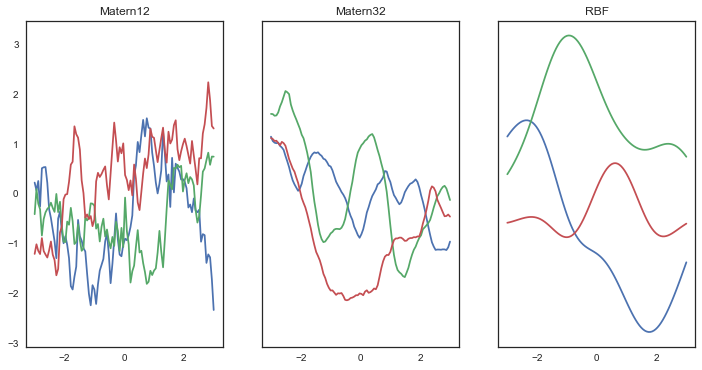
\includegraphics[width = 0.8\textwidth]{kernel_examples}
\end{figure}


The periodic is another class of stationary kernel. The variant used in this project follows MacKay 1998  \cite{mackay1998introduction}:

$$ k_p(t) = exp \bigg[ - \frac{1}{2}\sigma_i \big(\frac{sin(\frac{\pi}{\Delta}(t_i - t_i'))}{\ell} \big)^2 \bigg] $$

$\Delta$ is a periodicity paramter that can either be fit or set to a fixed anticipated value such as 52 for annual weekly data. $\ell$ is again the lengthscale parameter.\par


\subsection{Priors}

Gelman 2006 suggests using a student-t prior distribution restricted to be positive (a 'half-t') as a prior for variance parameters in hierarchical models \cite{gelman_2006}. Since variance is always positive it is acceptable and desirable to restrict the prior distribution to be non-negative as well. Flaxman 2014 used a standard student-t prior with 4 degrees of freedom on all parameters (not just variance). Both standard Normal $N \sim (0,1)$ and Student-T priors were considered here. The normal prior has less probability mass in its tails than the Student-t but is otherwise a close substitute. The Normal prior did sometimes lead to the optimization algorithm failing to find a credible set of parameter estimates, while the Student-T with degrees of freedom between 2 and 10 performed better. Increasing the variance on the prior distributions was another way to lower the probability of the optimizer failing, but it also led to dramatically increased runtimes in some cases.

\section{Methods for fitting LGCPs}

Solutions to the computational challenges in fitting LGCPs have advanced rapidly over the past five years. As mentioned earlier, the computational bottleneck for Gaussian Process models is the the n-by-n covariance matrix, which requires an $O(n^3)$ computation. Fitting a GP model as $n$ grows beyond a few thousand points is quite challenging \cite{gelman2013bayesian}. \par

 As recently as 2012 the best methods for fitting LGCP models involved variations of the Metropolis-Hastings sampling algorithm which were considered to be slow and highly inefficient in generating acceptable draws from the posterior distribution of the model \cite{murray_2012}. Advances in statistical computing have opened the door for several new model fitting methods, each with their own advantages and drawbacks.

\subsection{Variational Inference}

Variational Inference (VI) methods attempt to recover parameter estimates for a posterior distribution of interest by specifying a more tractable family of distributions and optimizing the resulting approximation using closed-form or computational methods. Usually the family of approximating distributions is denoted $Q$, and the optimization seeks to minimize the Kullback-Leiber divergence $KL[(\theta), p(\theta|y)]$ between $q(\theta)$ and the true posterior $p(\theta|y)$. \par

In the case of the LGCP with Poisson likelihood there is no direct closed-form solution because an intractable integral is involved. VI methods have in the past been limited by needing to make simplifying assumptions about the approximating distributions. Usually VI makes the 'mean-field' assumption (borrowed from physics), that the posterior can be approximated by the product of some number of existing distributions: $q(\theta_1,...,\theta_n)= \prod_j{q_j(\theta_j)}$. The mean-field assumption is especially unsuited for high-dimensional models like a Gaussian Process, but Tran and Blei characterize a Variational Gaussian Process method that avoids the assumption \cite{tran_2015}. GPflow - the package used for this project - uses the Variational Gaussian  for fitting \cite{GPflow2017}.\par

The major drawback of variational methods is there are no theoretical justifications for the accuracy of estimates produced because it is unclear and often unknowable how close the optimized approximation is to the true posterior distribution, where the $KL$ divergence term is a unitless and uninterpretable difference between the two that cannot be compared across models. Yao et., al. recently proposed Pareto-Improved-Importance-Sampling (PSIS) and Variational-Simulation-Based-Calibration (VSBC) methods for assessing whether a VI approximation ''worked'' \cite{yao_2018}.

\subsection{MCMC}

Markov Chain Monte Carlo (MCMC) sampling methods by contrast do have theoretical properties that ensure consistent estimation of the posterior distribution - at least  as the numbers of samples increases asympotically \cite{teng_2017}. MCMC methods are not a new development in themselves, but there have been breakthroughs both in MCMC algorithm design and computing power required to fit more complex models. The probablistic programming language Stan has been used for spatiotemporal modelling of causes of mortality using Gaussian Markov Random Field models, another potential alternative to LGCPs that may be appropriate for urban forecasting but are not considered here \cite{stan} \cite{foreman_2017}. In contrast to VI, MCMC also is capable of producing estimates for full posterior distributions for parameters of interest, rather than point estimate approximations. In the case of urban prediction and forecasting, access to full posterior estimates would offer much more probalistic information from which to draw uncertainty-based conclusions in a policy or administrative context.

\subsection{LaPlace Approximation}

Integrated Nested LaPlace Approximation (INLA) is an alternative to MCMC capable of fitting a LGCP \cite{illian_toolbox}. INLA works by approximating the distribution of each parameter around the mode of its posterior \cite{lindgren2015bayesian}. The marginal posteriors are calculated by numerically integrating over the parameters, followed by another approximation of the marginal posterior (hence the 'Nested' component of INLA). When the number of hyperparameters is relatively small, INLA is capable of quickly fitting a latent Gaussian field model - of which the LGCP is a special case \cite{rue2009approximate}. LGCP models usually assume a square grid structure for the spatial component in order to fit the model, but Simpson 2016 also fits LGCPs without relying on explicit grid structure \cite{simpson2016going}.


\section{Method Choice}

MCMC methods clearly offer desirable properties superior to VI methods, and full MCMC models similar to the ones considered here have been explored \cite{Flaxman2015FastHG}. However, their practical limitations made them somewhat burdensome to consider for this project. The most unfortunate drawbacks were that MCMC is very slow to fit in comparison with VI. In an attempt to draw a compromise between ease of experimentation and model reliability this project used VI methods under the knowledge that they may not produce the best results for practical use. Simple posterior checks were done to assess the results.


\section{Experiments}
\label{experiments}

Both long- and short-term forecasting experiments were considered, as well as both neighborhood level spatial granularity and a larger city level spatial scheme.

\todo{Table of SML term and city/nta/grid characteristics}


\subsection{GPflow}

GPflow is a Python package developed for fitting Gaussian Process models that takes advantage of the autodifferentiation abilities of Google's TensorFlow to generate Maximum-A-Posteriori (MAP) estimates of the posterior distribution \cite{GPflow2017} \cite{tensorflow2015-whitepaper}. All models are converted into tensors and passed to Tensorflow's optimization algorithms that can run on Graphics Processing Units (GPUs) for fast and efficient computation. This cuts the time needed for each iteration significantly compared to running on a CPU and also doesn't restrict the user to using conjugate distributions when specifying priors and likelihoods - a prerequisite for the LGCP model. GPflow is also capable of full Bayesian inference using Hamiltonian Monte Carlo (HMC).

\subsubsection{Custom Modifications}

While GPflow offers most of the settings required 'out-of-the-box', a few additional features had to be added independently. The base package does not offer the option for a Student-T prior, which was relatively easy to add by writing a new custom Student-T class to GPflow. The package also by default does not easily allow for decomposition of the different kernels' contribution to the parameter estimates. Finally, the GPflow implementation of Matern kernels often exhibit unstable behavior and, even after re-centering data. A small jitter was added to the Matern32 kernel in in order to reduce the chance of the Cholesky Decomposition failing. All modifications can be found in the appendix \todo(cite to appendix code).

\subsection{Kernel Choice}

Besides making a choice for or against stationarity, kernels also embed other assumptions about the model's

\section{Results}
\label{results}

Borrowing again from Flaxman 2014, the models were evaluated on a variant of $R^2$ that captures the reduction in variance from each model component. The error from predicting solely on the spatial expectation $e_s$ serves as a baseline for comparison:

$$ 1 - \frac{\sigma_{s,t}(n_{s,t}- \hat{n_{s,t}})^2}{\sigma_{s,t}(n_{s,t} - e_{s})^2}$$


\subsection{Long Term Predictions}

 Weekly traffic collision and injury data was aggregated to the level of New York City neighborhoods for this set of experiments. While data is available for the past five years, there appears to have been a reporting error for part of 2016 which made the year of data problematic for both model fitting and testing. It would have been ideal to fit the model based on multiple years of data leading up to the latest available data, but given the unreliable data the best alternative was fitting the LGCP on three years of data from July 2012 to July 2015, and leaving the following 52 weeks for out-of-sample prediction.  \par


 \begin{figure}[h!]
   \caption{A Gaussian Process fit to weekly pedestrian injuries in New York City from 2012 to 2015. The dotted line shows where out of sample prediction begins.}
   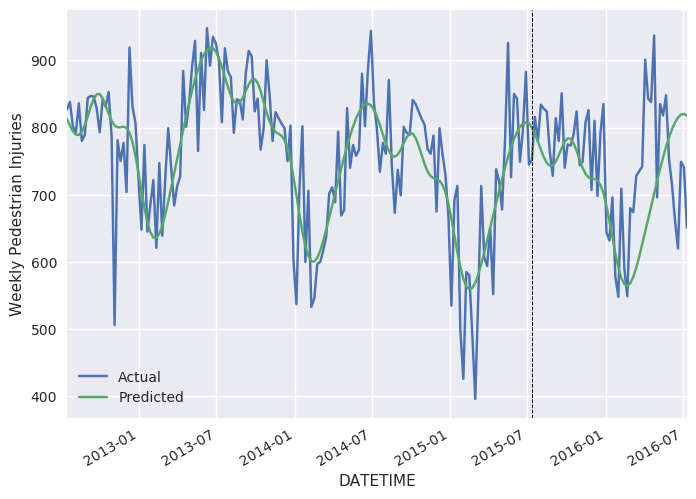
\includegraphics[width=0.5\textwidth]{citywide_predictions}
 \end{figure}

\todo{discussion of confidence?}

Since the kernel components are all additive they can provide an interpretable decomposition of the model components. There is clear annual periodicity in the model, which is also confirmed by the period parameter fitted being almost exactly 52. The linear kernel component also suggests a small downward long-term trend in pedestrian injuries.

\todo{table of parameters}


\begin{figure}[h!]
  \caption{}
  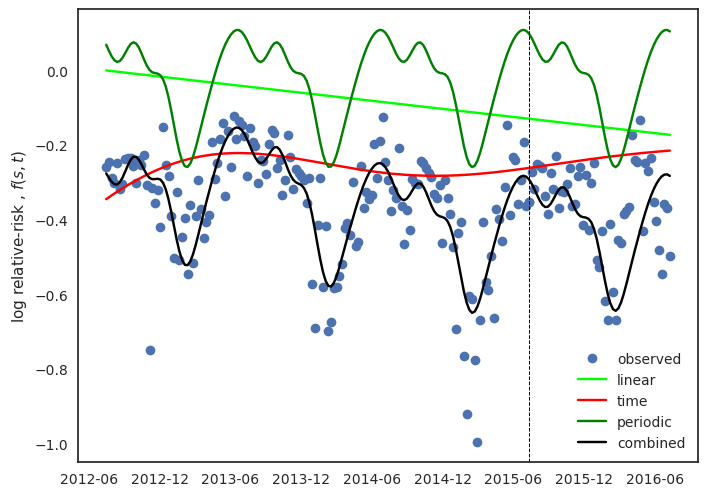
\includegraphics[width=0.5\textwidth]{citywide_var_decomp}
\end{figure}

 \todo{chart of data errors}


 \subsection{Neighborhood Predictions}

 Neighborhood level predictions of pedestrians injuries were added
 New York City defines official Neighborhood Tabulation Areas (NTAs), which were used as the geographic areas of interest. The model was fit on the 29 official NTAs in the borough of Manhattan using 52 weeks of weekly pedestrian injury data. The spatial component was calculated from the distance between centroids for each NTA. \par

 \begin{figure}[h!]
   \caption{Manhattan's 29 neighborhoods, with red dots indicating the centroid used for calculating distance.}
   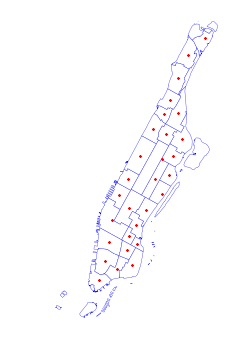
\includegraphics[width=0.5\textwidth]{mn_centroids}
 \end{figure}

 \begin{figure}[h!]
   \caption{Relative risk scores for Manhattan neighborhoods. Midtown is roughly twice as dangerous for pedestrians than Manhattan as a whole.}
   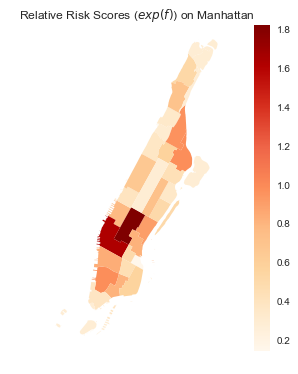
\includegraphics[width=0.5\textwidth]{mn_f_score_map}
 \end{figure}



 \todo{data example}
 \todo{NTA map}


\subsection{Short Term Forecasting}

\chapter{Discussion}
\label{discussion}

The goal of this research was to evaluate the value of spatiotemporal Gaussian Process models for applications in urban policy evaluation and forecasting, and some of the results are quite promising. Gaussian processes are capable of convincingly modelling the incidence of traffic collisions in various resolutions of urban environment. The citywide temporal model offers a decomposition of the inevitably noisy observed data into components which are directly useful to policymakers and far better predictors than a simple average, all while relying only on previously observed count data as an input. The LGCP model of traffic collisions decomposes a longer term 'secular' trend from short-term variability and yearly seasonality. The long term model however did have some statistical shortcomings, chiefly the ill-fitted credible intervals and poor $k$ score. This should caution against relying on the model for overly precise predictions over the long term. \par

Modelling the spatial heterogeneity between neighborhoods as well as across time also has many potential uses. The interpretation of the latent function $f_i$ at each location as a measure of relative risk is straightforward and easily applied for policy purposes. Again the decomposition of the kernel components allows for easy interpretation of the degree to which space and time contribute to the overall risk in each neighborhood, as well as being directly comparable to any other neighborhood. \par

The most ambitious modelling initiative was to attempt to forecast individual events at very high spatial detail, in some cases down to the space of one or two city blocks. This method offered better performance than normal autoregression when the lookback period was short while performing comparably to an AR(1) as the period was lengthened. The Reduction-in-Variance analysis suggest that the spatial distance component is valuable especially when timeseries data are otherwise sparse. It is also possible that a pure spatial model would perform better in this situation, based on how much of the Reduction-in-Variance is due to the spatial component.

\section{Methodological Issues}

\subsection{Zero Inflation}


The LGCP model as specified suffers when dealing with  sparse observations, which happens naturally when events are recorded at increasing levels of spatial and temporal granularity. When using a very small grid edge sizes of 500-1000ft, The model would often converge to a trivial constant relative risk prediction of $f(s,t)=1$ , which is equivalent to a prediction of $e_s$ at all points. Sometimes the approximation would fail to converge at all. It is possible the Poisson likelihood suffers from the 'zero-inflation' problem. With most grid and time points having no observations a majority of the time, a Poisson distribution does not have enough probability mass near zero to provide a good fit. An alternative likelihood like the Zero-Inflated Binomial may be better suited for very rare events. \par

\subsection{Unstable Inference}

The high PSIS-LOO scores of all the models is discouraging. This suggests potentially poor optimization results when fitting with Variational Inference. Using full posterior inference with Markov Chain Monte Carlo methods would assess whether the model fits from VI are problematic. GPflow does offer a Hamiltonian Monte Carlo sampling algorithm, but it is still experimental and also prone to instability. Using another probablistic programming language with reliable MCMC methods such as Stan's No-U-Turn Sampler (NUTS) would be more reliable and also likely more efficient than Hamiltonian Monte Carlo.


\subsection{Scalability vs. Reliable and Full Inference}

Another benefit of MCMC is that it will return estimates of full distributions for all model parameters. This would offer much more complete information for uncertainty-based decision making when using GP models for prediction and forecasting. For example, full distributions for each latent risk function $f(s,t)$ could be used to compare relative risk outcomes and allocate resources for e.g., traffic calming measures like additional enforcement based on an acceptable risk tolerance. \par

Gaussian Processes are slow to fit with MCMC, since the Cholesky Decomposition has to be done at every iteration of the algorithm. This makes doing full inference slow in some cases and prohibitively complex as the number of dimensions grows. There are some workarounds to this, such as exploiting Kronecker Algebra for fast computations \cite{flaxman_2015_FastKron}, but the dimensionality is still limited to the thousands. While this is more than enough for most applications it does prevent scaling local spatial analysis to cover an area the size of a city while making estimates for relatively small grid squares. One promising alternative is making use of Bochner's theorem, which guarantees any valid stationary kernel can be represented using a Fourier transform \cite{rasmussen_2005}:

$$ k(\mathbf{\tau})=\int_{\mathbb{R^D}}e^{2\pi i \mathbf{s}\mathbf{\tau}}d\mu(\mathbf{s}) $$

Hensman 2018 exploits this for a method called Variational Fourier Features that is capable of estimating high-dimensional models with millions of datapoints in minutes without specialized computing hardware \cite{hensman_vff}. Flaxman 2018 exploits Fourier features as well to apply a Poisson likelihood grid model for forecasting crime for the entire city of Portland, Oregon \cite{flaxman_2018}. Since the spatiotemporal LGCP models considered in this project assumed a stationary kernel by design they would be feasible candidates for using Variational Fourier Features while scaling to larger geographies. Avoiding relying on specialized GPU hardware would be another benefit.


\section{Other Potential Data Sources}

Other urban datasets may be just as- or even better suited to prediction using Guassian Processes. Many public issues where data are collected do not suffer from the sparsity issues of traffic collisions when making predictions at high resolution. Ubiqitious city annoyances like noise and pests are observed far more frequently than traffic collisions and would also benefit from reliable methods for prediction and comparative risk. Outside of the public sphere, taxi and ride-share vehicle demand are good candidates for heavily localized events which would benefit from granular forecasting.


\section{Potential for Bias}

 The data used for modelling in this project were deliberately limited to the count data of interest, without relying on supplementary predictive or controlling variables.  One obvious side effect of this choice that neverless bears stating directly is any bias in the data will be diligently reproduced in the predictions. Here 'bias' is meant in the sense of predictions skewed toward existing inaccuracies in the data provided rather than the technical definition of statistical bias.\par

This is especially relevant considering ongoing research into the performance of predictive algorithms when trained on data which had reporting bias. An illustrative example is a 2016 study of predictive policing systems in Oakland, California \cite{lum2016predict}. Lum and Isaac found that the proprietary algorithm provided by a private contractor replicated , rather than controlled for, reporting bias in the training data stemming from historical overpolicing of black Americans for drug offenses. The models used here have also been used for experiments using policing data \cite{flaxman_2014} \cite{flaxman_2018}. The risks of biased predictions based on biased data are not as visible outside of policing, but they should not be ignored when there is potential to practically apply these spatiotemporal models.

\section{Measuring Distance}

This project, like the previous research it was based on, relied on simple Euclidean distance in the spatial kernel. Euclidean distance is an excellent 'one-size-fits-all' distance measure for general use, but other measures may be even more suited for predicting events taking place on a street grid. Manhattan distance would be a first alternative, and there is also the potential to use the actual street grid for measuring distance, see \ref{AppendixA} for a representative example. This would also necessitate getting rid of the square grid structure, which would make the LGCP intractable \cite{teng_2017}. However, alternatives already exist and may be suitable for use in this case \cite{simpson2016going}. Finally, there is potential to use a distance measure that does not rely on geography at all; something like a social network could also be used as the spatial component.


\section{Future Work}

There are many possibilities for improvement and refinement. The most valuable would be to move to full Bayesian inference. It is possible to write one of the tested models in an MCMC friendly language such as Stan, which would be capable of generating posterior samples for all variables and parameters of interest rather than relying only on approximated point estimates, opening the door for explicit relative risk comparisons based on the modelled uncertainty. MCMC estimates would also provide a 'sanity check' on the variational approximations and potentially explain why model performance is sometimes poor or unstable. Practically speaking, moving to MCMC would also negate the need for a specialized computing environment with a GPU. if the MCMC results are promising, a further next step would be to experiment with scale by transfering the stationary models to Variational Fourier Features. With VFF it would become trivial to create grid models with high resolution that cover entire cities instead of just one neighborhood and fit them quickly on standard computer hardware.  \par


A good portion of the necessary data manipulations could also be automated and abstracted. Automating the creation of the spatial grid, aggregating counts, re-centering variables, and other mundane tasks would make it much easier to experiment on different datasets quickly and efficiently.


\section{Conclusion}

The goal of this research was to evaluate the feasibility of spatiotemporal prediction and forecasting using a model framework that would be relatively easy to use "out of the box" with only space and time data for each observation. Gaussian Process models are both theoretically and practically suitable in this case. The latent function structure of the Log Gaussian Cox Process provides direct estimates and predictions as well as a comparative statistic to gauge the relative prevalence of a phenomenona between places and times. \par

The experimental results show that the LGCP performs as well or better at prediction than a standard autoregression as measured by Mean Squared Error in long-, medium-, and short-term cases. The Reduction-in-Variance estimates show that the fitted models explain variations in spatial timeseries far better than relying on simple averages (an admittedly naive comparison), especially in the long-term model. The decomposed variance components also clearly delineate how time, space, seasonality, and long-term trends influence the total prediction. \par

While Gaussian Process models meet all the practical criteria for interpretable estimates and ease-of-use, the experiments also highlight some instability in fitting and unreliability in results. The worrisome PSIS-LOO scores as well as too-narrow credible intervals should not be ignored, especially when relying on variational inference methods that may not always suitably approximate the posterior distribution. \par

Still, Gaussian Process models are general and flexible enough to work with data at the city, neighborhood, and even hyperlocal level while also allowing flexible time inputs. There is potential to apply the same models to other uses of practical interest to urban planners, public safety officials, businesses, and anyone else who has some stake in an urban environment. Hopefully this project is a small step towards showing that 'cities are already smart.'

\endgroup


\begin{appendices}
\setcounter{subsection}{0}
\renewcommand\thesubsection{\Alph{subsection}}

\clearpage
\label{AppendixA}
\vspace{-1.75cm}
\section{Additional Figures}


\begin{figure}[h!]
  \centering
  \caption{The decomposition of contribution to total log risk for a high-risk grid square.}
  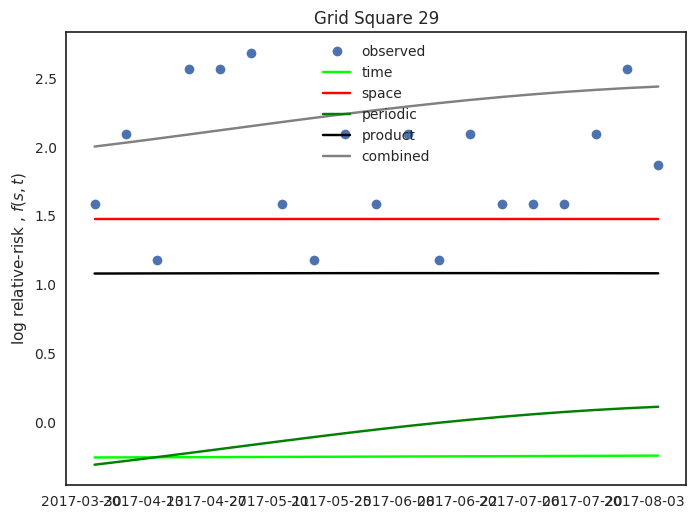
\includegraphics[width=\textwidth]{grid_var_decomp}
\end{figure}


 \begin{figure}[h!]
   \centering
     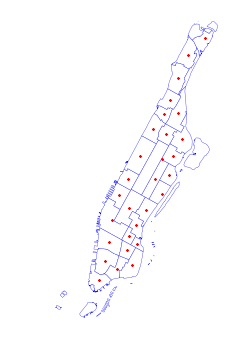
\includegraphics[\linewidth]{mn_centroids}
     \caption{Manhattan's 29 neighborhoods, with red dots indicating the centroid used for calculating distance.}
\end{figure}

\input{sections/appendices/appendixB}
%\input{sections/appendices/appendixC}

\end{appendices}


\backmatter

\begingroup
\bibliography{bibliography.bib}
\endgroup

\end{document}
